\documentclass{article}

%%%%%%%%%%%%%%%%%%% layout
\usepackage{indentfirst}
\setlength{\parindent}{2em}
% We will use NIPS submission format
\usepackage{../common/nips13submit_e,times}

% for hyperlinks
\usepackage{hyperref}
\usepackage{url}
% For figures
\usepackage{graphicx}
\usepackage{subfigure}
% math packages
\usepackage{amsmath}
\usepackage{amsfonts}
\usepackage{amsopn}
\usepackage{ifthen}
\usepackage{natbib}
\usepackage{enumerate}
\usepackage{booktabs}
\usepackage{fancyhdr}
\usepackage{fancyvrb}
\usepackage{float}
\usepackage[utf8]{inputenc}
\usepackage[top=3cm,bottom=3cm,right=3cm,left=3cm]{geometry}
% appendix
\usepackage{appendix}


\usepackage{tikz}
\usetikzlibrary{mindmap,trees}

\usepackage{CJKutf8}
% from epfml.
% numbers
\newcommand{\0}{\mathbf{0}}
\newcommand{\1}{\mathbf{1}}
\newcommand{\Identm}{\mathbf{I}}

% bold vectors
\renewcommand{\aa}{\mathbf{a}}
\newcommand{\bb}{\mathbf{b}}
\newcommand{\cc}{\mathbf{c}}
\newcommand{\dd}{\mathbf{d}}
\newcommand{\ee}{\mathbf{e}}
\newcommand{\ff}{\mathbf{f}}
\let\ggg\gg
\renewcommand{\gg}{\mathbf{g}}
\newcommand{\hh}{\mathbf{h}}
\newcommand{\ii}{\mathbf{i}}
\newcommand{\jj}{\mathbf{j}}
\newcommand{\kk}{\mathbf{k}}
\let\lll\ll
\renewcommand{\ll}{\mathbf{l}}
\newcommand{\mm}{\mathbf{m}}
\newcommand{\nn}{\mathbf{n}}
\newcommand{\oo}{\mathbf{o}}
\newcommand{\pp}{\mathbf{p}}
\newcommand{\qq}{\mathbf{q}}
\newcommand{\rr}{\mathbf{r}}
\renewcommand{\ss}{\mathbf{s}}
% \newcommand{\tt}{\mathbf{t}}
\newcommand{\uu}{\mathbf{u}}
\newcommand{\vv}{\mathbf{v}}
\newcommand{\ww}{\mathbf{w}}
\newcommand{\xx}{\mathbf{x}}
\newcommand{\yy}{\mathbf{y}}
\newcommand{\zz}{\mathbf{z}}

% bold matrices
\newcommand{\mA}{\mathbf{A}}
\newcommand{\mB}{\mathbf{B}}
\newcommand{\mC}{\mathbf{C}}
\newcommand{\mD}{\mathbf{D}}
\newcommand{\mE}{\mathbf{E}}
\newcommand{\mF}{\mathbf{F}}
\newcommand{\mG}{\mathbf{G}}
\newcommand{\mH}{\mathbf{H}}
\newcommand{\mI}{\mathbf{I}}
\newcommand{\mJ}{\mathbf{J}}
\newcommand{\mK}{\mathbf{K}}
\newcommand{\mL}{\mathbf{L}}
\newcommand{\mM}{\mathbf{M}}
\newcommand{\mN}{\mathbf{N}}
\newcommand{\mO}{\mathbf{O}}
\newcommand{\mP}{\mathbf{P}}
\newcommand{\mQ}{\mathbf{Q}}
\newcommand{\mR}{\mathbf{R}}
\newcommand{\mS}{\mathbf{S}}
\newcommand{\mT}{\mathbf{T}}
\newcommand{\mU}{\mathbf{U}}
\newcommand{\mV}{\mathbf{V}}
\newcommand{\mW}{\mathbf{W}}
\newcommand{\mX}{\mathbf{X}}
\newcommand{\mY}{\mathbf{Y}}
\newcommand{\mZ}{\mathbf{Z}}
\newcommand{\mLambda}{\mathbf{\Lambda}}

% caligraphic
\newcommand{\cA}{\mathcal{A}}
\newcommand{\cB}{\mathcal{B}}
\newcommand{\cC}{\mathcal{C}}
\newcommand{\cD}{\mathcal{D}}
\newcommand{\cE}{\mathcal{E}}
\newcommand{\cF}{\mathcal{F}}
\newcommand{\cG}{\mathcal{G}}
\newcommand{\cH}{\mathcal{H}}
\newcommand{\cJ}{\mathcal{J}}
\newcommand{\cK}{\mathcal{K}}
\newcommand{\cL}{\mathcal{L}}
\newcommand{\cM}{\mathcal{M}}
\newcommand{\cN}{\mathcal{N}}
\newcommand{\cO}{\mathcal{O}}
\newcommand{\cP}{\mathcal{P}}
\newcommand{\cQ}{\mathcal{Q}}
\newcommand{\cR}{\mathcal{R}}
\newcommand{\cS}{\mathcal{S}}
\newcommand{\cT}{\mathcal{T}}
\newcommand{\cU}{\mathcal{U}}
\newcommand{\cV}{\mathcal{V}}
\newcommand{\cX}{\mathcal{X}}
\newcommand{\cY}{\mathcal{Y}}
\newcommand{\cW}{\mathcal{W}}
\newcommand{\cZ}{\mathcal{Z}}

\newcommand{\lin}[1]{\ensuremath{\left\langle #1 \right\rangle}}
\newcommand{\abs}[1]{\left\lvert#1\right\rvert}
\newcommand{\norm}[1]{\left\lVert#1\right\rVert}

% random variables
\newcommand{\E}[1]{{\rm E}\left[#1\right] }     %expectation
\newcommand{\EE}[2]{{\rm E}_{#1}\left[#2\right] } %expectation
\newcommand{\prob}[1]{{\rm Pr}\left[#1\right] }
\newcommand{\Prob}[2]{{\rm Pr}_{#1}\left[#2\right] }

% macros
\newcommand{\R}{\mathbb{R}}

\newcommand{\A}{\mathcal{A}}
\newcommand{\B}{\mathcal{B}}
\newcommand{\C}{\mathcal{C}}
\newcommand{\D}{\mathcal{D}}
\newcommand{\G}{\mathcal{G}}
\newcommand{\Hc}{\mathcal{H}}
\newcommand{\Ic}{\mathcal{I}}
\newcommand{\Lc}{\mathcal{L}}
\newcommand{\Oc}{\mathcal{O}}
\newcommand{\M}{\mathcal{M}}
\newcommand{\N}{\mathcal{N}}
\newcommand{\Sc}{\mathcal{S}}
\newcommand{\T}{\mathcal{T}}
\newcommand{\U}{\mathcal{U}}
\newcommand{\V}{\mathcal{V}}
\newcommand{\X}{\mathcal{X}}
\newcommand{\Y}{\mathcal{Y}}
\newcommand{\W}{\mathcal{W}}

\newcommand{\av}{\boldsymbol{a}}
\newcommand{\bv}{\boldsymbol{b}}
\newcommand{\cv}{\boldsymbol{c}}
\newcommand{\dv}{\boldsymbol{d}}
\newcommand{\ev}{\boldsymbol{e}}
\newcommand{\fv}{\boldsymbol{f}}
\newcommand{\gv}{\boldsymbol{g}}
\newcommand{\hv}{\boldsymbol{h}}
\newcommand{\iv}{\boldsymbol{i}}
\newcommand{\jv}{\boldsymbol{j}}
\newcommand{\kv}{\boldsymbol{k}}
\newcommand{\lv}{\boldsymbol{l}}
\newcommand{\mv}{\boldsymbol{m}}
\newcommand{\nv}{\boldsymbol{n}}
\newcommand{\ov}{\boldsymbol{o}}
\newcommand{\pv}{\boldsymbol{p}}
\newcommand{\qv}{\boldsymbol{q}}
\newcommand{\rv}{\boldsymbol{r}}
\newcommand{\sv}{\boldsymbol{s}}
\newcommand{\tv}{\boldsymbol{t}}
\newcommand{\uv}{\boldsymbol{u}}
\newcommand{\wv}{\boldsymbol{w}}
\newcommand{\xv}{\boldsymbol{x}}
\newcommand{\yv}{\boldsymbol{y}}
\newcommand{\zv}{\boldsymbol{z}}

\newcommand{\ellv}{\boldsymbol{\ell}}


\newcommand{\Xv}{\boldsymbol{X}}
\newcommand{\Yv}{\boldsymbol{Y}}
\newcommand{\Zv}{\boldsymbol{Z}}

%

\newcommand{\ym}{\boldsymbol{y}}


\newcommand{\Am}{\boldsymbol{A}}
\newcommand{\Bm}{\boldsymbol{B}}
\newcommand{\Cm}{\boldsymbol{C}}
\newcommand{\Dm}{\boldsymbol{D}}
\newcommand{\Em}{\boldsymbol{E}}
\newcommand{\Fm}{\boldsymbol{F}}
\newcommand{\Gm}{\boldsymbol{G}}
\newcommand{\Hm}{\boldsymbol{H}}
\newcommand{\Ivm}{\boldsymbol{I}}
\newcommand{\Lm}{\boldsymbol{L}}
\newcommand{\Mm}{\boldsymbol{M}}
\newcommand{\Pm}{\boldsymbol{P}}
\newcommand{\Rm}{\boldsymbol{R}}
\newcommand{\Sm}{\boldsymbol{S}}
\newcommand{\Tm}{\boldsymbol{T}}
\newcommand{\Um}{\boldsymbol{U}}
\newcommand{\Vm}{\boldsymbol{V}}
\newcommand{\Wm}{\boldsymbol{W}}
\newcommand{\Xm}{\boldsymbol{X}}
\newcommand{\Ym}{\boldsymbol{Y}}
\newcommand{\Zm}{\boldsymbol{Z}}

\newcommand{\id}{\boldsymbol{\iota}}
\newcommand{\diag}{\mbox{$\mbox{diag}$}}

%
\newcommand{\Xmt}{\tilde{\Xm}}
\newcommand{\Cmt}{\tilde{\Cm}}

%
\newcommand{\alphav}{\boldsymbol{\alpha}}
\newcommand{\betav}{\boldsymbol{\beta}}
\newcommand{\epsilonv}{\boldsymbol{\epsilon}}
\newcommand{\thetav}{\boldsymbol{\theta}}
\newcommand{\muv}{\boldsymbol{\mu}}
\newcommand{\Sigmav}{\boldsymbol{\Sigma}}
\newcommand{\Omegav}{\boldsymbol{\Omega}}

\newcommand{\nablav}{\boldsymbol{\nabla}}
\newcommand{\deltav}{\boldsymbol{\delta}}
\newcommand{\kappav}{\boldsymbol{\kappa}}
\newcommand{\chiv}{\boldsymbol{\chi}}
\newcommand{\xiv}{\boldsymbol{\xi}}
\newcommand{\piv}{\boldsymbol{\pi}}
\newcommand{\phiv}{\boldsymbol{\phi}}
\newcommand{\varsigmav}{\boldsymbol{\varsigma}}
\newcommand{\sigmav}{\boldsymbol{\sigma}}
\newcommand{\zetav}{\boldsymbol{\zeta}}
%
\newcommand{\KL}{\text{KL}}
\newcommand{\NLL}{\text{NLL}}
\newcommand{\BLEU}{\text{BLEU}}
\newcommand{\RNN}{\text{RNN}}
\newcommand{\LSTM}{\text{LSTM}}
\newcommand{\enc}{\text{enc}}
\newcommand{\dec}{\text{dec}}
\newcommand{\score}{\text{score}}
\newcommand{\softmax}{\text{softmax}}
\newcommand{\onehot}{\text{one\_hot}}
\newcommand{\sgn}{\text{sgn}}
\newcommand{\Elias}{\text{Elias}}
\newcommand{\Code}{\text{Code}}
\newcommand{\threshold}{\text{threshold}}


\newcommand{\costfunc}{\mathcal{L}}
\newcommand{\deriv}[2]{\frac{\partial{#1}}{\partial{#2}}}
\newcommand{\secondderiv}[2]{\frac{\partial^2{#1}}{\partial{#2}^2}}

% symbol
\DeclareMathOperator*{\argmin}{arg\,min}
\DeclareMathOperator*{\argmax}{arg\,max}
\DeclareMathOperator*{\argsup}{arg\,sup}
\newcommand{\indep}{\rotatebox[origin=c]{90}{$\models$}}


% continue the numbering based on previous list.
\newcounter{saveenumi}
\newcommand{\seti}{\setcounter{saveenumi}{\value{enumi}}}
\newcommand{\conti}{\setcounter{enumi}{\value{saveenumi}}}



%%%%%%%%%%%%%%%%%%% configure note.
\usepackage[textwidth=4.3cm]{todonotes}
\newcommand{\tao}[1]{\todo[color=red!20,size=\footnotesize]{T: #1}{}}

%%%%%%%%%%%%%%%%%%% highlight something.
\usepackage{xcolor}
\usepackage{soul}
\newcommand{\mathcolorbox}[2]{\colorbox{#1}{$\displaystyle #2$}}
\newcommand{\hlfancy}[2]{\sethlcolor{#1}\hl{#2}}

%%%%%%%%%%%%%%%%%%% begin the document.
\nipsfinalcopy
\begin{document}
\begin{CJK}{UTF8}{gbsn}
\CJKindent

\title{缺陷检测项目进度}
\author{林涛 刘俊峰}
\date{2019年 6月 26}
\maketitle


%\section{Template 模版}


\begin{abstract}
	\hspace{2em}
	项目报告主要分为两大块“分类模型”和“检测模型”,每一块从总体的项目思维导图、项目的关键节点和相关实验结果分析三个部分组成。
  深度学习框架为pytorch,编程语言为python,模型训练设备为双GPU 1080Ti。
\end{abstract}

%\chapter{图像分类}
\section{图像分类}
当前项目为灰度图像的分类模型构建,一共有七种分类类别。评价指标包括Accuracy和Confusion Matrix。
\subsection{项目思维导图}

\pagestyle{empty}
\begin{figure}[htb]
\centering
\begin{tikzpicture}[scale=0.8]
  \path[mindmap,concept color=black,text=white]
    node[concept] {图像分类项目}
    [clockwise from=0]

    % 节点1
    child[concept color=green!50!black] {
      node[concept] {1.数据采集}
      [clockwise from=100]
      child { node[concept] {分类类别数量:单个图像多标签} }
      child { node[concept] {数据的纯度} }
    }
    % 节点2
    child[concept color=blue!80!white] {
      node[concept] {2.数据预处理}
      [clockwise from=40] % 旋转的角度
      child { node[concept] {放缩(resize)} }
      child { node[concept] {旋转,平移} }
      child { node[concept] {归一化(正态分布,均匀分布)}}
      child { node[concept] {亮度,锐度,对比度}}
    }
    child[concept color=red] {
      node[concept] {3.模型训练}
      [clockwise from=-70]
      child [concept color=orange]{
      node[concept] {a.模型结构}
      [clockwise from=-30]
      child { node[concept] {基础模型} }
      child { node[concept] {速度} }
      child { node[concept] {精度} }
       }
      child[concept color=orange]{
      node[concept] {b.调参}
      [clockwise from=-100]
      child { node[concept] {参数初始化}}
      child { node[concept] {学习率}}
      child { node[concept] {weight decay}}
      child { node[concept] {batchsize}}
       }
      child [concept color=orange]{
       node[concept] {c.增加泛化能力}
       [clockwise from=-180]
       child {node[concept]{优化器}}
       child {node[concept]{Regularization}}
       child {node[concept]{增加数据的质量和数量}}
       }
     }
    child[concept color=orange] {
    node[concept] {4.模型预测}
    [clockwise from=150]
    child {node[concept]{评价指标(Accuracy/confusion matrix)}}
    child {node[concept]{过拟合/欠拟合}}
    };
\end{tikzpicture}
\end{figure}


%\newpage
\subsection{项目关键节点}
\subsubsection{模型收敛}
原始图片格式为tif的710*710灰度图,模型发散。后剪切为480*480,剪切依据为图像周围的像素点不在分类图像的特征区域。模型初步筛选的结果在小节~\ref{clip}
原因分析:

\subsubsection{图像放缩和归一化}
考虑到模型的batch size比较小,训练时间长。故图片放缩到300*300大小,经ResNet网络测试该策略的有效性(精度提升1-2个点)。当时有过FPN22网络进行测试,实验结果没有及时保存,后期测试添加!具体的分辨率与精度和batch size之间的关系在小节\ref{300*300}。
根据数据集计算出mean和std,对读取的480*480图像进行放缩(300*300)和Normalization,最终的输入图片可视化结果Figure~\ref{fig:nor-img}
原因分析:

\subsubsection{缓解过拟合}

\subsubsection{迁移学习}

\subsubsection{合并分类类别}


%\newpage
\subsection{实验细节}

\subsubsection{改进一:图像裁剪}\label{clip}
原始图片和剪切之后的图片对比Figure~\ref{fig:origin-clip},直接剪切中心特征部分。
\begin{figure}[!ht]
    \centering
    \subfigure[原始图片]{
        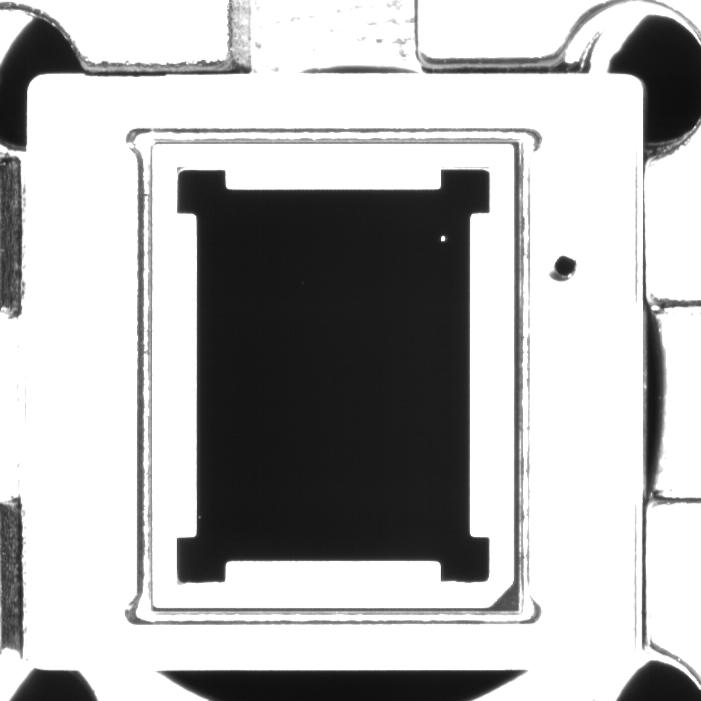
\includegraphics[width=0.5\textwidth,]{figures/origin-img.jpg}
        \label{fig:clip-img}
    }
    \hfill
    \subfigure[剪切图片]{
        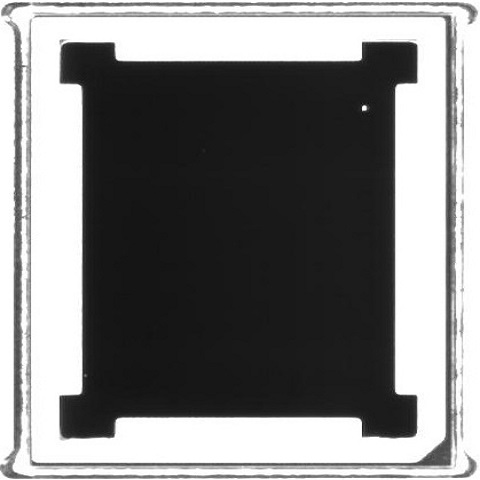
\includegraphics[width=0.3\textwidth,]{figures/clip-img.jpg}
        \label{fig:clip-img}
    }
    \caption{图像剪切}
    \label{fig:origin-clip}
\end{figure}
模型测试结果如Table~\ref{tab:model-test}

\begin{table}[!ht]
\centering
\begin{tabular}{|c|c|c|c|c|}
\hline
model      & train\_acc & test\_acc & valid\_acc & parameters(M) \\ \hline
ResNet20   & 0.99       & 0.807     & 0.79       & 0.28          \\ \hline
DenseNet20 & 0.77       & 0.688     & 0.407      & 0.04          \\ \hline
FPN22      & 1.0        & 0.623     & 0.64       & 10.27         \\ \hline
\end{tabular}
\caption{模型对比}
\label{tab:model-test}
\end{table}


\begin{figure}[!ht]
    \centering
    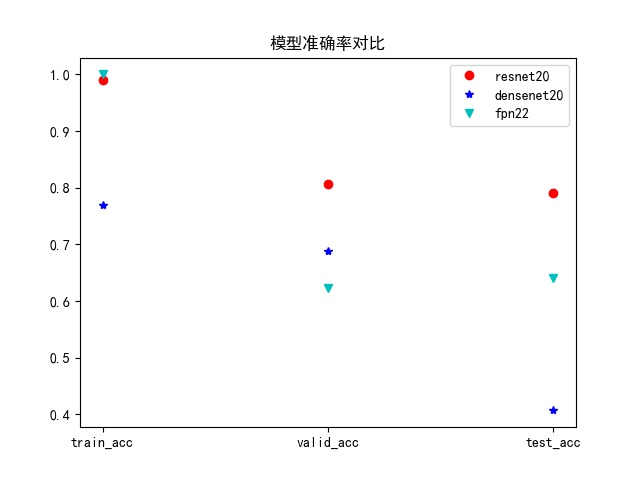
\includegraphics[width=0.8\textwidth]{figures/model_vs_acc.jpg}
    \caption{模型准确率对比}
    \label{vs-acc}
\end{figure}


\subsubsection{改进二:图像放缩和归一化}\label{300*300}

\begin{figure}[!ht]
    \centering
    \subfigure[batch-size vs resolution]{
        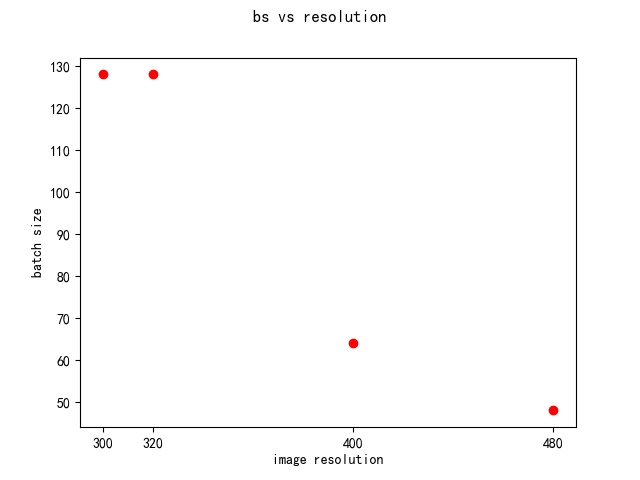
\includegraphics[width=0.45\textwidth,]{figures/bs-vs-resolution.jpg}
        \label{fig:clip-img}
    }
    \hfill
    \subfigure[accuracy vs resolution]{
        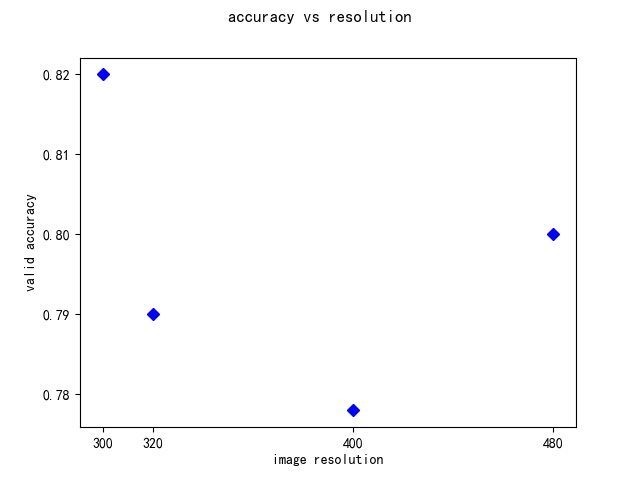
\includegraphics[width=0.45\textwidth,]{figures/accuracy-vs-resolution.jpg}
        \label{fig:clip-img}
    }
    \caption{image resize}
    \label{fig:img-resize}
\end{figure}

\begin{figure}[!ht]
    \centering
    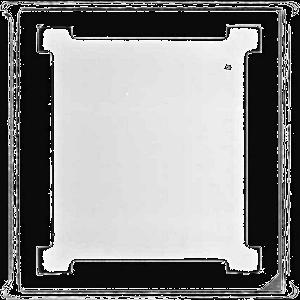
\includegraphics[width=0.4\textwidth]{figures/normalization.jpg}
    \caption{Normalization}
    \label{nor-img}
\end{figure}


\end{CJK}
\end{document}
